\documentclass[border=4pt]{standalone}
\usepackage{pgfplots}
\pgfplotsset{compat=1.18}

\begin{document}
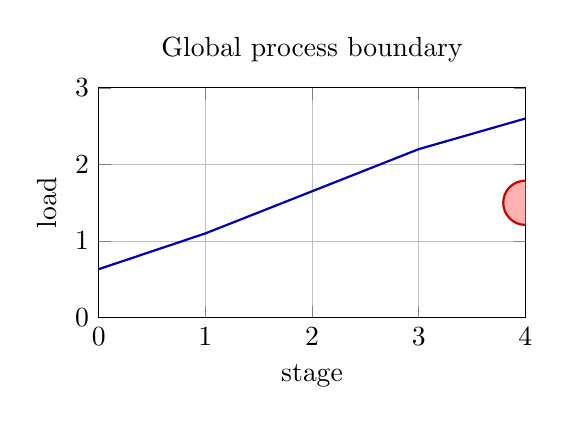
\begin{tikzpicture}
  \begin{axis}[
    width=7cm,
    height=4.5cm,
    xmin=0, xmax=4,
    ymin=0, ymax=3,
    enlargelimits=false,
    clip mode=global,
    grid=major,
    title={Global process boundary},
    xlabel={stage}, ylabel={load}
  ]
    \addplot[blue!70!black,thick] coordinates {(-0.5,0.4) (1,1.1) (3,2.2) (4.5,2.8)};
    \filldraw[red!80!black,fill=red!30,thick] (axis cs:4,1.5) circle (8pt);
  \end{axis}
\end{tikzpicture}
\end{document}
